\subsection{Gram-Schmidt Orthogonalization Process}\label{subsec:Gram-Schmidt_Orthogonalization}
\begin{definition}[Span]\label{def:Span}
  The \emph{span} of a vector or set of vectors, is a linear combination of all possible vectors.
  For example, if $S = \lbrace u_{1}, u_{2} \rbrace$, then $\Span(S) = \lbrace c_{1}u_{1} + c_{2}u_{2} : c_{1}, c_{2} \in \RealNumbers \rbrace$.
\end{definition}

\begin{definition}[Projection]\label{def:Vector_Projection}
  The \emph{projection} of a vector onto another is the amount of one vector that is in the same direction as another.
  It is denoted $\Proj{u_{2}}{u_{1}}$, and is said ``the projection of $u_{2}$ on $u_{1}$''.
  It is defined as:
  \begin{equation}\label{eq:Vector_Projection}
    \Proj{u_{2}}{u_{1}} = \frac{u_{2} \cdot u_{1}}{u_{1} \cdot u_{1}} u_{1}
  \end{equation}
\end{definition}

\begin{definition}[Rejection]\label{def:Vector_Rejection}
  The \emph{rejection} of a vector from another vector is the amount that one vector is \textbf{not} in the same direction as another, in an orthogonal fashion.
  This can be seen graphically in \Cref{fig:Vector_Projection_Rejection}.
  It is denoted $\Rej{u_{2}}{u_{1}}$, and is said ``the rejection of $u_{2}$ from $u_{1}$''.
  If is defined as:
  \begin{equation}\label{eq:Vector_Rejection}
    \begin{aligned}
      \Rej{u_{2}}{u_{1}} &= u_{2} - \frac{u_{2} \cdot u_{1}}{u_{1} \cdot u_{1}} u_{1} \\
      \Rej{u_{2}}{u_{1}} &= u_{2} - \Proj{u_{2}}{u_{1}}
    \end{aligned}
  \end{equation}
\end{definition}

\begin{figure}[h!tbp]
  \centering
  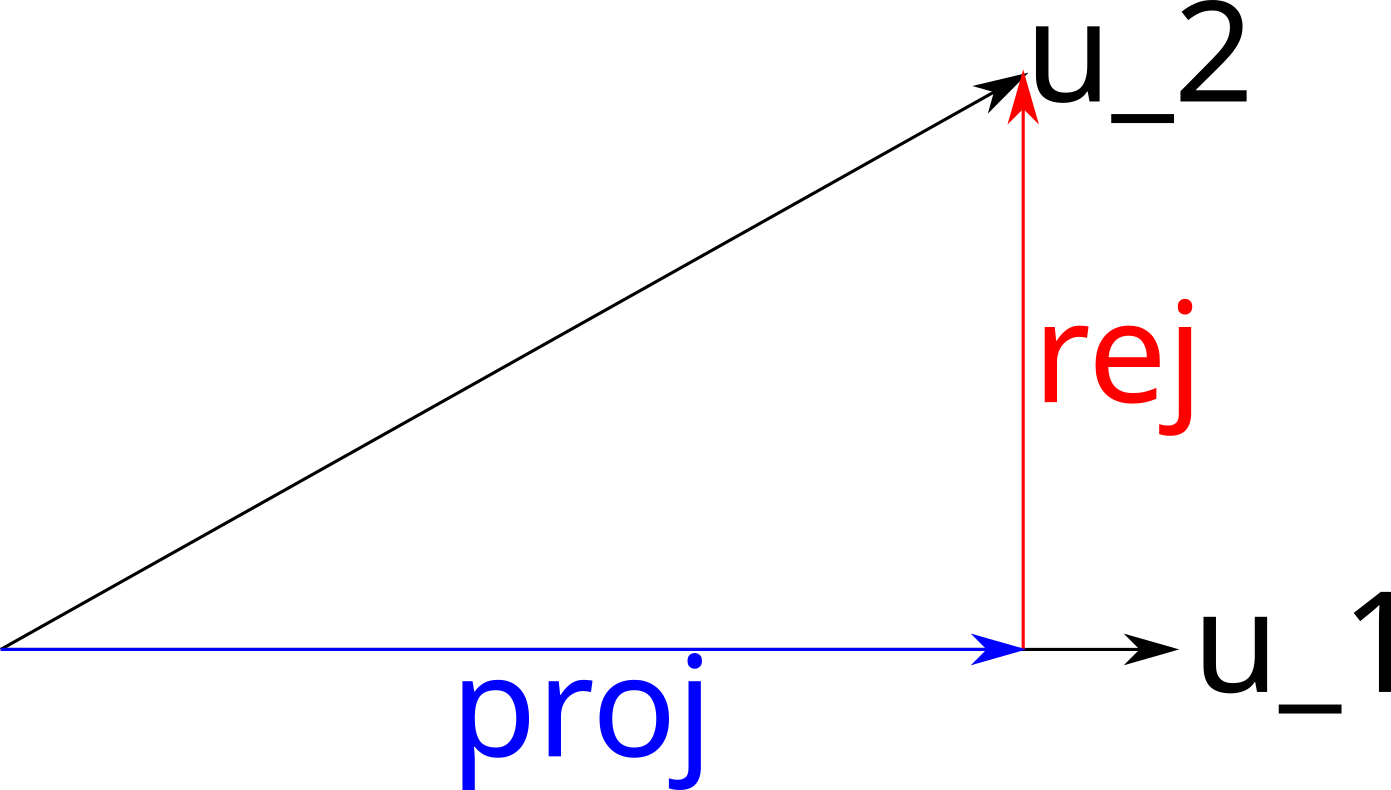
\includegraphics[scale=0.50]{./Vector_Projection_Rejection.png}
  \caption{Vector Projection and Rejection}
  \label{fig:Vector_Projection_Rejection}
\end{figure}

\begin{theorem}[Gram-Schmidt Orthogonalization Process]\label{thm:Gram-Schmidt_Orthogonalization}
  Given $m$ \nameref{def:Linearly_Independent} vectors in $\RealNumbers^{n}$ ($m$ vectors, each with $n$ components),
  \begin{equation*}
    S = \lbrace u_{1}, u_{2}, \ldots, u_{m} \rbrace, \: n \geq m
  \end{equation*}

  To find $V = \lbrace v_{1}, v_{2}, \ldots, v_{m} \rbrace$ orthogonal vectors where $\Span(V) = \Span(S)$.

  We can find such vectors by repeatedly using the \nameref{def:Vector_Rejection} of the original vector from the first orthogonal vector.
  So, the process boils down to:
  \begin{equation}\label{eq:Gram-Schmidt_Orthogonalization}
    \begin{aligned}
      v_{1} &= u_{1} \\
      v_{2} &= u_{2} - \Rej{u_{2}}{v_{1}} \\
      &= u_{2} - \frac{u_{2} \cdot v_{1}}{v_{1} \cdot v_{1}} v_{1} \\
      v_{3} &= u_{3} - \frac{u_{3} \cdot v_{1}}{v_{1} \cdot v_{1}} v_{1} - \frac{u_{3} \cdot v_{2}}{v_{2} \cdot v_{2}} v_{2} \\
      &\vdots \\
      v_{m} &= u_{m} - \frac{u_{m} \cdot v_{1}}{v_{1} \cdot v_{1}} v_{1} - \cdots - \frac{u_{m} \cdot v_{m-1}}{v_{m-1} \cdot v_{m-1}} v_{m-1}
    \end{aligned}
  \end{equation}
\end{theorem}


%%% Local Variables:
%%% mode: latex
%%% TeX-master: "../../Math_333-MatrixAlg_ComplexVars-Reference_Sheet"
%%% End:
